\documentclass[a4paper, openany, 12pt]{article}

%% подключаем стандарт библиографии
\bibliographystyle{gost71u}

%% для "Abstract" в классе book
% \newenvironment{abstract}{}{}
% \usepackage{abstract}

%% подключаем преамбулу: в ней содержится подключение всех необходимых пакетов
%% Работа с русским языком
\usepackage{cmap}			 % поиск в PDF
\usepackage{mathtext} 		 % русские буквы в формулах
\usepackage[T2A]{fontenc}	 % кодировка
\usepackage[utf8]{inputenc}	 % кодировка исходного текста
\usepackage[russian]{babel}	 % локализация и переносы

%% Пакеты для работы с математикой
\usepackage{amsmath,amsfonts,amssymb,amsthm,mathtools}
\usepackage{icomma}

%% Нумерация формул (опционально)
%\mathtoolsset{showonlyrefs=true} % показывать номера только у тех формул, на которые есть \eqref{} в тексте.
%\usepackage{leqno}               % нумерация формул слева

%% Шрифты
\usepackage{euscript}	 % шрифт "Евклид"
\usepackage{mathrsfs}    % красивый мат. шрифт

%% Некоторые полезные макросы для дебага (в случае недоверия авторам шаблона)
\makeatletter
\newcommand\thefontsize{The current font size is: \f@size pt} % пример: \section{\thefontsize}
\makeatother

%% Настройка размеров шрифтов
\makeatletter
\setlength{\headheight}{28pt}
%% TODO: мне не удалось разобраться, как грамотно подбирать второе число в 
%% \@setfontsize\*, но ряд эксппериментов показывает, что "10" выравнивает текст весьма прилично :)
\renewcommand\Huge{\@setfontsize\Huge{14pt}{10}}
\renewcommand\huge{\@setfontsize\huge{14pt}{10}}
\renewcommand\Large{\@setfontsize\Large{14pt}{10}}
\renewcommand\large{\@setfontsize\large{12pt}{10}}
\makeatother

%% Поля (геометрия страницы)
\usepackage[left=3cm,right=1.5cm,top=2cm,bottom=2cm,bindingoffset=0cm]{geometry}

%% Русские списки
\usepackage{enumitem}
\makeatletter
\AddEnumerateCounter{\asbuk}{\russian@alph}{щ}
\makeatother

%% Работа с картинками
\usepackage{caption}
\captionsetup{justification=centering} % центрирование подписей к картинкам
\usepackage{graphicx}                  % вставки рисунков
\graphicspath{{images/}{images2/}}     % папки с картинками
\setlength\fboxsep{3pt}                % отступ рамки \fbox{} от рисунка
\setlength\fboxrule{1pt}               % толщина линий рамки \fbox{}
\usepackage{wrapfig}                   % обтекание рисунков и таблиц текстом

%% Работа с таблицами
\usepackage{array,tabularx,tabulary,booktabs} % дополнительная работа с таблицами
\usepackage{longtable}                        % длинные таблицы
\usepackage{multirow}                         % слияние строк в таблице

%% Красная строка
\setlength{\parindent}{2em}

%% Интервалы
\linespread{1}
\usepackage{multirow}

%% TikZ
\usepackage{tikz}
\usetikzlibrary{graphs,graphs.standard}

%% Верхний колонтитул
\usepackage{fancyhdr}
\pagestyle{fancy}

%% Перенос знаков в формулах (по Львовскому)
\newcommand*{\hm}[1]{#1\nobreak\discretionary{}{\hbox{$\mathsurround=0pt #1$}}{}}

%% Дополнительно
\usepackage{float}   % добавляет возможность работы с командой [H] которая улучшает расположение на странице
\usepackage{gensymb} % красивые градусы
\usepackage{caption} % пакет для подписей к рисункам, в частности, для работы caption*
\usepackage{listings} % пакет для листингов с кодом
\lstset{              % настройки для лисингов с кодом
basicstyle=\small\ttfamily,
columns=flexible,
breaklines=true
}

% Hyperref (для ссылок внутри  pdf)
\usepackage[unicode, pdftex]{hyperref}

% Отступ перед первым абзацем в каждом разделе
\usepackage{indentfirst}

\DeclareMathOperator*{\argmax}{arg\,max}
\DeclareMathOperator*{\argmin}{arg\,min}

\usepackage{fancyvrb}

\lstdefinestyle{mypython}{
    language=Python,
    basicstyle=\ttfamily\small,
    keywordstyle=\color{blue},
    commentstyle=\color{gray}\itshape,
    stringstyle=\color{orange!80!black},
    showstringspaces=false,
    breaklines=true,
    frame=single,
    numbers=none,
    backgroundcolor=\color{gray!5},
    upquote=true,
    inputencoding=utf8,
    literate=
    {а}{{\cyra}}1 {б}{{\cyrb}}1 {в}{{\cyrv}}1 {г}{{\cyrg}}1 {д}{{\cyrd}}1
    {е}{{\cyre}}1 {ё}{{\cyryo}}1 {ж}{{\cyrzh}}1 {з}{{\cyrz}}1 {и}{{\cyri}}1
    {й}{{\cyrishrt}}1 {к}{{\cyrk}}1 {л}{{\cyrl}}1 {м}{{\cyrm}}1 {н}{{\cyrn}}1
    {о}{{\cyro}}1 {п}{{\cyrp}}1 {р}{{\cyrr}}1 {с}{{\cyrs}}1 {т}{{\cyrt}}1
    {у}{{\cyru}}1 {ф}{{\cyrf}}1 {х}{{\cyrh}}1 {ц}{{\cyrc}}1 {ч}{{\cyrch}}1
    {ш}{{\cyrsh}}1 {щ}{{\cyrshch}}1 {ъ}{{\cyrhrdsn}}1 {ы}{{\cyrery}}1
    {ь}{{\cyrsftsn}}1 {э}{{\cyrerev}}1 {ю}{{\cyryu}}1 {я}{{\cyrya}}1
    {А}{{\CYRA}}1 {Б}{{\CYRB}}1 {В}{{\CYRV}}1 {Г}{{\CYRG}}1 {Д}{{\CYRD}}1
    {Е}{{\CYRE}}1 {Ё}{{\CYRYO}}1 {Ж}{{\CYRZH}}1 {З}{{\CYRZ}}1 {И}{{\CYRI}}1
    {Й}{{\CYRISHRT}}1 {К}{{\CYRK}}1 {Л}{{\CYRL}}1 {М}{{\CYRM}}1 {Н}{{\CYRN}}1
    {О}{{\CYRO}}1 {П}{{\CYRP}}1 {Р}{{\CYRR}}1 {С}{{\CYRS}}1 {Т}{{\CYRT}}1
    {У}{{\CYRU}}1 {Ф}{{\CYRF}}1 {Х}{{\CYRH}}1 {Ц}{{\CYRC}}1 {Ч}{{\CYRCH}}1
    {Ш}{{\CYRSH}}1 {Щ}{{\CYRSHCH}}1 {Ъ}{{\CYRHRDSN}}1 {Ы}{{\CYRERY}}1
    {Ь}{{\CYRSFTSN}}1 {Э}{{\CYREREV}}1 {Ю}{{\CYRYU}}1 {Я}{{\CYRYA}}1
}

\lstset{style=mypython}

\usepackage{minted}

\begin{document}
    %% титульник
    \begin{center}
    %% *название института*
    \large\textbf{Министерство образования и науки Российской Федерации \\
    Московский физико-технический институт (государственный
    университет)} \\
    \vspace{1cm}

    %% *факультет/физтех-школа*
    Физтех-школа прикладной математики и информатики \\
    %% *название базовой кафедры и лаборатории*
    %% в случае ненадобности можно удалить
    Лаборатория машинного интеллекта\\

    \vspace{3em}

    Выпускная квалификационная работа бакалавра
\end{center}

\begin{center}
    \vspace{\fill}
    %% *название вашей работы*
    \LARGE{Эффективное дообучение больших языковых моделей в задаче выделения информации из контекста }

    \vspace{\fill}
\end{center}


\begin{flushright}
    \textbf{Автор:} \\
    Студент 131 группы \\
    Вицын Семён Сергеевич \\
    \vspace{2em}
    \textbf{Научный руководитель:} \\
    Алексей Владимирович Гончаров \\
    \vspace{2em}
    \textbf{Научные консультанты:} \\
    Глеб Моргачев \\
    Алексей Меркулов \\
    Валентин Шишков \\
\end{flushright}

\vspace{7em}

\begin{center}
    %% *лого*
    
\includegraphics[width=100 pt]{MIPT_logo.jpg}\\
    Москва \the\year{}
\end{center}

%% выключаем отображение номера для этой страницы (титульник)
\thispagestyle{empty}

\newpage
\setcounter{page}{2}
\fancyfoot[c]{\thepage}
%% *надпись над верхним колонтинулом*
%% в случае ненадобности можно удалить
\fancyhead[L]{\fontsize{10}{12} \selectfont Эффективное дообучение больших языковых моделей в задаче выделения информации из контекста}
\fancyhead[R]{}

    %% аннотоция
    \fontsize{14}{20}\selectfont
    \begin{center}
    \large{Эффективное дообучение больших языковых моделей в задаче выделения информации из контекста} \\
\end{center}

\begin{center}
    \large\textit{Вицын Семён Сергеевич} \\[1 cm]
\end{center}

Современные подходы к улучшению языковых моделей всё чаще основываются на Retrieval Augmented Generation (RAG), отходя от прямого дообучения под конкретные задачи. Однако, несмотря на универсальность метода, он сопряжён с рядом трудностей. Данная работа посвящена изучению этих проблем, а также методам адаптаций языковых моделей для задач RAG и способам оценки их эффективности.

\vfill

\newpage
    %% содержание
    \tableofcontents{}
    \newpage

    \section{Введение}
\label{sec:Intro} \index{Chapter1}

В последние годы большие языковые модели (LLM) достигли значительного прогресса. Такие архитектуры уже сейчас способны эффективно решать широкий круг задач. В число таких задач входят: перевод, обработка и суммаризация текстовых данных, автоматизация бизнес-процессов через использование чат-ботов, а также многое другое. Однако действительно высоких результатов удается достигать только на моделях, в которых количество параметров исчисляется десятками и сотнями миллиардов. В то же время их разработка и поддержка требуют огромных вычислительных ресурсов, а среди качественных проблем главными остаются фактологические ошибки моделей и их неспособность адаптироваться к динамически изменяющимся данным.

При создании систем, способных поддерживать актуальность знаний в определенной предметной области, на сегодняшний день чаще всего используют метод Retrieval Augmented Generation (RAG) \cite{RAG}. Для этого подхода требуется формирование и поддержание документационных индексов, содержащих всю необходимую информацию по целевому домену. Наиболее частым сценарием применения подобных систем является Question-Answering (QA), когда задачей модели является генерация ответа на запрос пользователя с учетом документационной базы. Для этого в контекст генерации интегрируются релевантные фрагменты, извлечённые на основе пользовательского вопроса. 

В классической постановке такую архитектуру можно разделить на 4 ключевых блока:

\begin{enumerate}

  \item \textbf{\textit{Система предобработки данных.}}
  
    Компонент, который отвечает за обработку и разбиение исходных документов на более мелкие фрагменты (чанки). На этом этапе дополнительно может быть произведена очистка или обогащение метаданными (например, указание источника или номера главы).
    
  \item \textbf{\textit{Retriever.}}
  
    Часть системы, выполняющая задачу поиска релевантных фрагментов документации на основе пользовательского запроса. Может быть реализована с помощью классических статистических подходов, таких TF-IDF или BM25. На практике чаще всего представляют собой нейросетевую модель, отображающую текстовые фрагменты в векторное пространство высокой размерности для последующего поиска семантически близких фрагментов. 
    
  \item \textit{\textbf{Системы векторного хранения и поиска.}}
  
    Специализированное хранилище, оптимизированное для эффективного поиска по векторным представлениям. Оно индексирует чанки, преобразованные retriever’ом, и поддерживает операции поиска по метрике близости. Популярными решениями являются Qdrant (полноценная векторная база данных) и FAISS (библиотека для эффективного векторного поиска).

  \item \textit{\textbf{Генератор.}}
  
    Языковая модель, в контекст генерации которой подается запрос пользователя и извлеченные ранее текстовые фрагменты. Обогащение контекста документацией позволяет LLM генерировать ответ с учётом актуальной информации.
  
\end{enumerate}

Общая схема работы алгоритма изображена на рис. \ref{RAG pipeline intro}.

\begin{figure}[ht!]
    \centering
    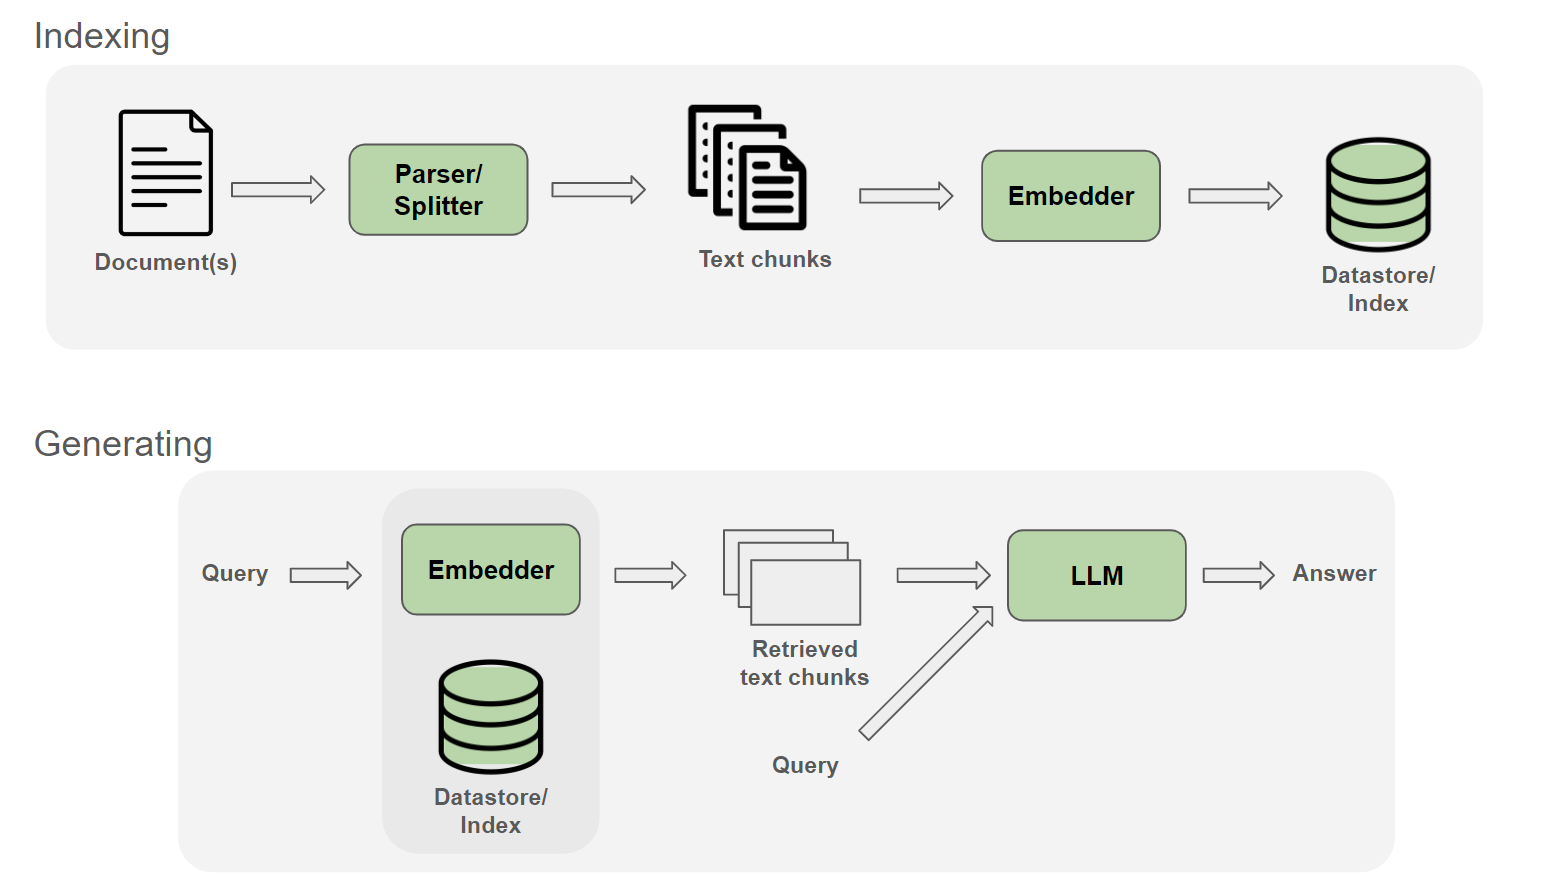
\includegraphics[scale=0.4]{images/rag_intro.png}
    \caption{Схема RAG pipeline.}
    \label{RAG pipeline intro}
\end{figure}

\newpage

% Этот подход крайне популярен и имеет множество вариаций. Так, например, алгоритм Graph RAG \cite{Graph_RAG} дополняет базовый принцип RAG за счёт извлечения сущностей и построения графа отношений по всему корпусу. В результате при поиске релевантного контекста можно осуществлять поиск по иерархически структурированному графу знаний. 

% Еще одним распространненным подходом является добавление модели ранжирования. Ее задачи состоит в изменении порядка извлеченных документов(лучшие впереди) и убирании избыточных документов. Продолжение этой идеи можно найти в работе <<RAG-Fusion: a New Take on Retrieval-Augmented Generation>> \cite{}   

Работа фокусируется на использовании языковых моделей в качестве интеллектуальных ассистентов для работы с обширными массивами документации. Многие современные компании активно разрабатывают и внедряют подобные системы в свою инфраструктуру. 

Технология полезна как для внутренних сотрудников компаний благодаря оперативному доступу к релевантной информации, так и для улучшения взаимодействия внешних пользователей с продуктом. При формировании ответа ключевым фактором является его фактологичность и корректность.

Несмотря на подтверждённую эффективность и широкое распространение, архитектура RAG имеет ряд ограничений, связанных с качеством её генеративной компоненты. В научной литературе выделяются две ключевые проблемы:

\begin{enumerate}

  \item \textbf{\textit{Генерация ответов на основе ложного контекста.}}
  
    Согласно исследованию <<Large Language Models Can Be Easily Distracted by Irrelevant Context>> \cite{irrelevant_retrieve}, некорректный контекст в RAG может вызывать <<галлюцинации>> модели, основанные на ложной или нерелевантной информации. Возможны даже ситуации, когда LLM могла самостоятельно ответить на поставленный вопрос, однако при добавлении дополнительного контекста, ответ становился неверным (рис. \ref{Hallucinations}).

    \begin{figure}[h!]
        \centering
        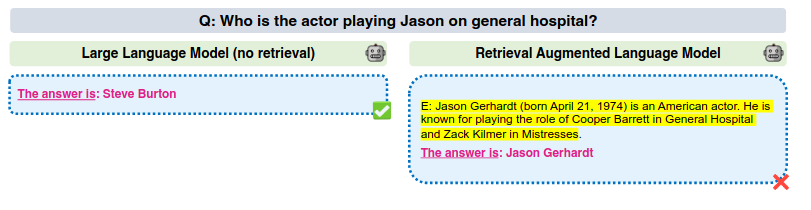
\includegraphics[scale=0.5]{images/hallucinations.png}
        \caption{Неверный ответ из-за нерелеватного контекста, взято из \cite{irrelevant_retrieve_ralm}}
        \label{Hallucinations}
    \end{figure}

  \item \textbf{\textit{Зависимость от позиции релевантной информации.}}

    При использовании RAG-систем для генерации ответов часто применяют модели, поддерживающие обработку расширенных контекстов. Данный подход позволяет потенциально передать больше релевантной информации. И хотя с технической точки зрения нет проблемы в реализации архитектур с большим или даже неограниченным контекстом, однако качество ответов моделей в таких сценариях значительно ухудшается. 

    Применительно к задаче извлечения информации эта проблема подробно описана в статье <<Lost in the Middle: How Language Models Use Long Contexts>> \cite{lost_in_the_middle}. Результаты исследования показывают, что LLM по умолчанию плохо справляются с извлечением информации из большого объёма разрозненных документов, фокусируясь преимущественно на информации в начале и в конце (рис. \ref{Lost in the middle}). Это приводит к снижению качества генерации, вплоть до уровня ниже, чем при отсутствии вспомогательных документов.

    \begin{figure}[h!]
        \centering
        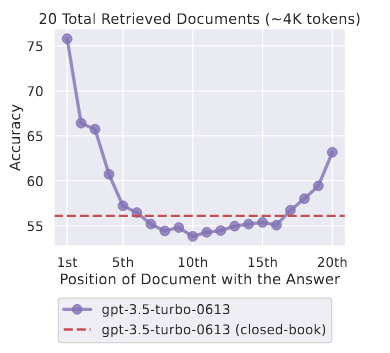
\includegraphics[scale=0.9]{images/Lost_in_the_middle.png}
        \caption{Качество ответа в зависимости от положения релевантной информации в контексте, взято из \cite{lost_in_the_middle}.}
        \label{Lost in the middle}
    \end{figure}
  
\end{enumerate}

Таким образом, возникает необходимость дообучения языковых моделей для повышения качества выделения информации из контекста. Для LLM критически важно не только извлекать полезные сведения из всего контекста генерации, но и иметь возможность находить и игнорировать шумовые или противоречивые фрагменты.

Важно отметить, что в рамках RAG-архитектур языковые модели выполняют функцию контекстуальных агрегаторов, синтезируя ответ на основе предварительно отобранной информации. На практике данную задачу, в отличие от классического QA, можно считать упрощенной, так как модель фокусируется не на генерации, а на структурировании ответа, что снижает требования к её «пониманию» изложенной информации.

Данная особенность открывает возможность оптимизации вычислительных ресурсов через применение компактных архитектур (объёмом 1-2 млрд параметров) при условии их специализированной адаптации под RAG-сценарии. Сохранение производительности в таких условиях достигается за счёт узкой специализации модели и усовершенствованных методов работы с контекстом.

Цель данного исследования — анализ, разработка и комбинация эффективных подходов дообучения LLM в сочетании с методами оценки качества генерации для задач RAG в условиях ограниченных вычислительных ресурсов.

\newpage
 %% Введение
    \section{Предметная область}
\label{subject_area} \index{Chapter2}

Введем определения, используемые в данной работе:


\begin{table}[ht]
\centering
\caption{Нотация}
\fontsize{12}{14}\selectfont
\renewcommand{\arraystretch}{1.2} % Увеличиваем высоту строк
\begin{tabularx}{\textwidth}{>{\centering\arraybackslash}m{3cm} >{\centering\arraybackslash}m{3cm} >{\centering\arraybackslash}X}
\toprule
\textbf{Термин} & \textbf{Обозначение} & \textbf{Описание} \\
\midrule
Корпус документов & $\mathcal D = \{d_i\}_{i=1}^{|\mathcal D|}$ & Множество объектов, где $d_i$ — фрагмент документации после этапа предобработки. \\
\midrule
Retriever & $f_{\phi}, f_{\psi}$ & Отображения текстовых данных в $\mathbb{R}^m$ с параметрами $\phi$ и $\psi$. Отображение $f_{\phi}$ для пользовательских запросов, а $f_{\psi}$ для документов.\\
\midrule
Метрика близости & $Sim(q,d)$ & Семантическая близость между запросом и документом. \\
\midrule
Generator (LLM) & $g_\theta$ & Отображение, параметризованное $\theta$. \\
\midrule
Запрос & $q$ & Пользовательский запрос. \\
\midrule
Контекст & $c$ & Контекст запроса. \\
\midrule
Ответ & $a$ & Целевой ответ. \\
\midrule
QA датасет & $X = \{X_i\}_{i=1}^{|X|}$ & Набор объектов, где $X_i$ = $(q_i, c_i, y_i)$. \\
\bottomrule
\end{tabularx}
\end{table}


Обучением модели будем называть процесс построения оптимального отображения, минимизирующего целевую функцию потерь.

Обучаемыми параметрами модели - параметры отображения, которые могут изменяться в ходе процесса обучения модели для получения оптимального результата.

\subsection{Большая языковая модель}
\label{subsec:math} \index{Chapter2!Math}

С точки зрения формальной математической постановки большая языковая модель это отображение, моделирующее вероятностное распределение следующего токена (символа или части слова) в текста, т.е. $g_\theta: \mathcal V^{\!*} \mapsto [0, 1]^{|\mathcal V|}$, где $\mathcal V$ фиксированный словарь.

Вероятность последовательности токенов $(x_1, \ldots, x_{T})$ факторизуется авторегрессионно:

\begin{equation}
    P_{\theta}(x_1, \ldots, x_{T}) = \prod_{t=1}^{T} P_{\theta}(x_t \mid x_{<t}) \textit{, где $g_{\theta}(x_{\leq t}) = P_{\theta}(\cdot \mid x_{\leq t})$}
\end{equation}

Обучение производится на большом корпусе $D = \{(x_1^{(i)}, \ldots, x_{T_i}^{(i)}\}_{i=1}^{N}$ через вычисление оценки максимального правдоподобия, путем минимизации среднего отрицательного логарифма правдоподобия (NLL loss):

\begin{equation}
    \mathcal{L}_{LM}(\theta) = - \frac{1}{N} \sum_{i=1}^N \sum_{t=1}^{T_i} log P_{\theta}(x_t^{(i)} \mid x_{<t}^{(i)})
    \label{generative_loss}
\end{equation}

Этот этап обычно называют предварительным обучением (pretrain). На нём модель <<получает>> основные знания о мире и оптимизируется для правдоподобного продолжения текстов. 

Следующим этапом является обучение на датасетах, составленных из инструкционных пар $D = \{I^{(i)}, R^{(i)}\}_{i=1}^{N} \textit{, где}$ 

\begin{itemize}
    \item $I^{(i)} = (l_1^{(i)}, \ldots, l_{L_i}^{(i)})$ - описание задачи на естественном языке.

    \item $R^{(i)} = (r_1^{(i)}, \ldots, r_{T_i}^{(i)})$ - ожидаемый ответ.
\end{itemize}

В данном случае задачей для LLM ставится генерация R. В частности функция потерь приобретает вид:

\begin{equation}
    \mathcal{L}_{SFT}(\theta) = - \frac{1}{N} \sum_{i=1}^N \sum_{t=1}^{T_i} log P_{\theta}(r_t^{(i)} \mid l_1^{(i)}, \ldots, l_{L_i}^{(i)} ,r_{<t}^{(i)})
\end{equation}

Этот этап называется Instruct Tuning или же Supervised Finetuning (SFT). Он необходим для адаптации модели к выполнению запросов, описанных на ествественном языке.  

Частным случаем инструкционного обучения является question-answering на датасете X:

\begin{equation}
    \mathcal{L}_{QA}(\theta) = - \frac{1}{|X|} \sum_{i=1}^X \sum_{t=1}^{T_i} log P_{\theta}(a_t^{(i)} \mid q^{(i)}, c^{(i)} ,a_{<t}^{(i)})
\end{equation}


\subsection{Retriever и генерация в RAG}
\label{subsec:rag} \index{Chapter2!RAG}

Как упоминалось ранее, в архитектуре RAG за создание информативных векторных представлений отвечает отдельный Retriever модуль. Формально, он задается как отображение $f: \mathcal T \mapsto \mathbb{R}^m$, где $\mathcal T$ - пространство текстов. Такие модели также называют эмбеддерами(embedder), а создаваемые ими представления эмбеддингами (embedding), они играют важную роль во множества задач машинного обучения. Ключевым требованием для информативности является:

\begin{itemize}
    \item $f(x) \approx f(y)$, если тексты $x$ и $y$ схожи по смыслу.
    \item $f(x) \not\approx f(y)$, если тексты $x$ и $y$ различны по смыслу.
\end{itemize}

Cемантическую близость полученных векторов чаще всего вычисляется по формуле косинусной меры близости или скалярного произведения:
\begin{equation}
   Similarity(q, d_i) = \langle f_{\phi}(q) \; , \; f_{\psi}(d_i) \rangle = f_{\phi}(q)^{\top} f_{\psi}(d_i)
\end{equation}

Принцип работы изображен на рис. \ref{retrieval}.

\begin{figure}[h!]
    \centering
    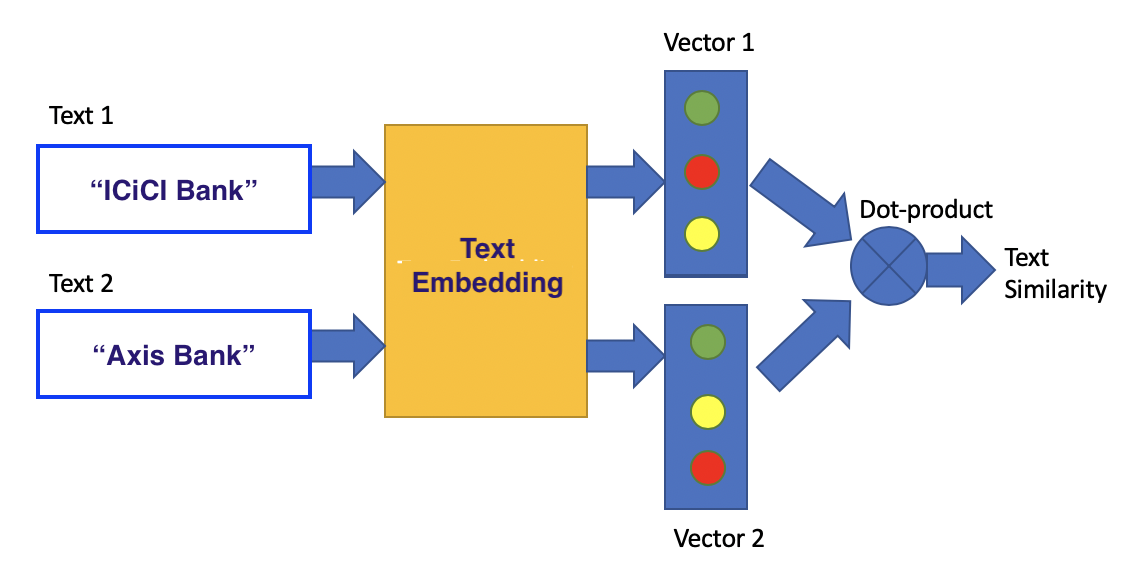
\includegraphics[scale=0.8]{./images/embedder.png}
    \caption{\protect\hypertarget{image1}{Алгоритм поиска метрики близости.}}
    \label{retrieval}
\end{figure}

Обучение retriever модели как правило основано на contrastive learning, когда для каждого запроса $q$ есть разметка, состоящая из целевого документа $d^{+}$ и набора нерелевантных документов $d^{-} = (d_1^{-}, \ldots, d_l^{-})$, а задачей является увеличение близости векторных представлений для $q$ и $d^{+}$, одновременно с уменьшением для $q$ и $d^{-}$.

Тогда вероятность релевантности документа $d \in \mathcal D$ к запросу $q$ оценивается как: 

\begin{equation}
    P(d \mid q) = \frac{exp(\langle f_{\phi}(q) \; , \; f_{\psi}(d) \rangle)}{\sum_{d' \in D}exp(\langle f_{\phi}(q) \; , \; f_{\psi}(d') \rangle)}
\end{equation}

А функция потерь на 1 объекте имеет вид:

\begin{equation}
    \mathcal{L}_{Retrieval} = -log P(d^{+} \mid q) = - log \frac{exp(\langle f_{\phi}(q) \; , \; f_{\psi}(d^{+}) \rangle)}{\sum_{d' \in D}exp(\langle f_{\phi}(q) \; , \; f_{\psi}(d') \rangle)}
    \label{retrieval_loss}
\end{equation}

При последующей генерации ответов языковая модель использует несколько наиболее вероятных документов. Другими словами, в качестве контекста для генерации LLM используются top-K фрагментов с наибольшей метрикой близости к запросу:

\begin{equation}
   c = \argmax_{\{{d_i}\}_{i=1}^K} \sum_{i=1}^K Similarity(q, d_i).
\end{equation}

\subsection{Архитектуры моделей}
\label{subsec:language_model} \index{Chapter2!Language model}


% Такая архитектура способна замечать более тонкие смысловые связи между запросом и документом, что зачастую повышает качество поиска. Однако, в то же время, нельзя гарантировать полную релевантность найденных документов.

В задачах Natural Language Processing (NLP) большое распространение получили трансформерные архитектуры, представленные в работы <<Attention Is All You Need>> \cite{transformer} (рис. \ref{transformer}).

\begin{figure}[ht!]
    \centering
    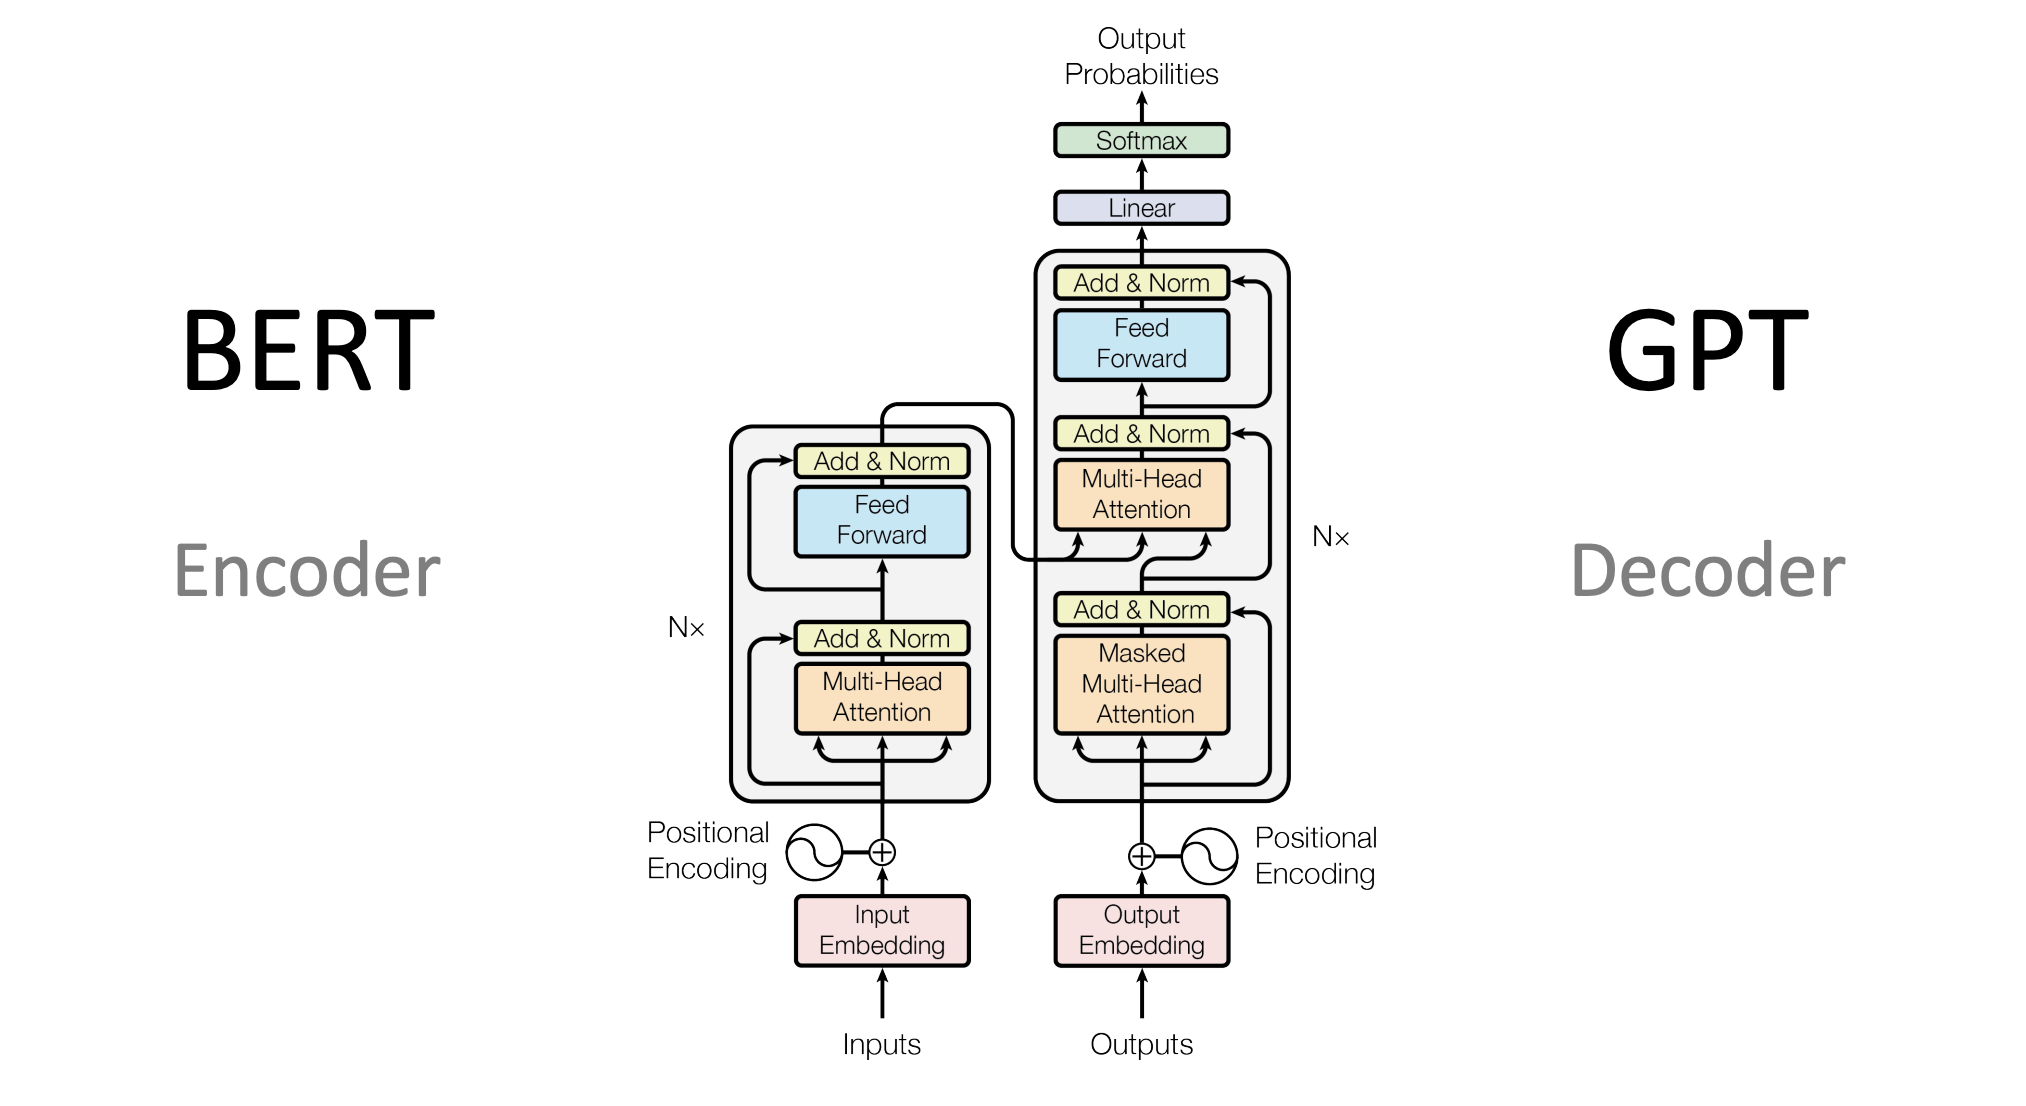
\includegraphics[scale=0.45]{images/transformers.png}
    \caption{Encoder-Decoder архитектура трансформер, оригинальное изображение взято из \cite{transformer}.}
    \label{transformer}
\end{figure}

Ключевой особенностью оригинальной архитектуры является представление в виде encoder-decoder пары, а также добавление механизма внимания, который учитывает влияние каждого элемента последовательности на текущий. Формально, self-attention вычисляется следующим образом:
\begin{equation}
    Attention(Q, K, V) = softmax(\frac{Q K^{\top}}{\sqrt{d_k}})V
\end{equation}
где $Q, K, V$ -- это матрицы запросов (queries), ключей (keys) и значений (values) соответственно, а $d_k$ -- размерность векторного пространства представлений.

Механизм внимания позволяет модели эффективно обрабатывать длинные текстовые последовательности ценой большей вычислительной сложности. Данная работа ограничивается рассмотрением только трансформерных архитектур. 

Дальнейшие исследования показали, что для генеративных задач наибольшую эффективность показывают gpt-подобные decoder-only архитектуры, обученные на кросс-энтропийной функции потерь (\ref{generative_loss}). 

Для embedder модели чаще всего применяются bert-подобные encoder-only архитектуры, обученные на контрастивную функцию потерь (\ref{retrieval_loss}).


% В частности, будем использовать открытые предобученные инструкционные модели. После этапа языкового моделирования на большом объеме данных они дополнительно обучаются на задачах, требующих следовать определенным инструкциям. Это необходимо для адаптации модели к формату вопрос-ответ, а также улучшению качества генерации при специализированном запросе.



\subsection{Метод Low-Rank Adaptation (LoRA)}
\label{subsec:lora} \index{Chapter2!LoRA}

Для эффективной адаптации языковой модели к целевой задаче в условиях ограничения вычислительных ресурсов чаще всего применяется метод низкоранговой адаптации \cite{LoRA}. Идея заключается в обновление исходных параметров $\mathbf{W}$ путём их заморозки и добавления $\Delta \mathbf{W}$, состоящего из низкорангового разложения (рис. \ref{lora}):

\begin{equation}
    \Delta \mathbf{W} = \mathbf{B}\mathbf{A}, \textit{где:}
\end{equation}

\begin{itemize}
    \item $\Delta \mathbf{W} \in R^{d \times k}$ -- матрица адаптации того же размера, что и исходная замороженная матрица весов $\mathbf{W}$.
    \item $\mathbf{B} \in \mathbb{R}^{d \times r}$, $\mathbf{A} \in \mathbb{R}^{r \times k}$ -- обучаемые матрицы.
    \item $r \ll \min(d, k)$ -- ранг разложения.
\end{itemize}

\begin{figure}[ht!]
    \centering
    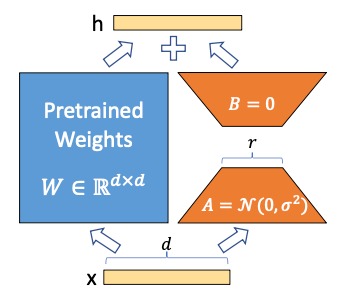
\includegraphics[scale=0.65]{images/lora_good.png}
    \caption{LoRA адаптер, изображение из \cite{LoRA}.}
    \label{lora}
\end{figure}

\noindentИтоговый слой модели действует следующим образом:
\begin{equation}
    W'(x) = h = \mathbf{W}x + \frac{\alpha}{r} \mathbf{B}\mathbf{A}x, \text{где $\alpha$ это гиперпараметр масштабирования.}
\end{equation}


\noindentИнициализация параметров:
\begin{itemize}
    \item $\mathbf{A} \sim \mathcal{N}(0, \sigma^2).$
    \item $\mathbf{B} = \mathbf{0}$ (нулевая инициализация).
\end{itemize}



\noindentСреди преимуществ метода можно выделить
\begin{itemize}
    \item Параметрическая эффективность (обучения 0.5-2\% от размера исходных параметров).
    \item Снижение риска катастрофического забывания.
    \item Высокая скорость обучения.
\end{itemize}



\subsection{Методы оценки качества}
\label{subsec:scoring_theory} \index{Chapter2!Scoring theory}

\subsubsection{ROUGE}
\label{subsec:rouge} \index{Chapter6!rouge}

ROUGE (Recall-Oriented Understudy for Gisting Evaluation) - серия метрик, предложенная в работе <<ROUGE: A Package for Automatic Evaluation of Summaries>> \cite{ROUGE} для оценки качества решения задачи суммаризации текста. 

Пусть есть 2 текста - сгенерированный $G$ и целевой $R$. Разобъем их на униграммы (отдельные слова), тогда определены следующие метрики:

\begin{equation}
    \textit{ROUGE-1 Precision} = \frac{\textit{Количество совпадающих униграм в $G$ и $R$}}{\textit{Количество униграм в G}}
\end{equation}

\begin{equation}
    \textit{ROUGE-1 Recall} = \frac{\textit{Количество совпадающих униграм в $G$ и $R$}}{\textit{Количество униграм в R}}
\end{equation}

\begin{equation}
    \textit{ROUGE-1 F1-score} = 2\frac{\textit{precision $\cdot$ recall}}{\textit{precision + recall}}
\end{equation}

Аналогично определяются метрики ROUGE-N, путём разбиения текста на $n$-граммы. Метрики ROUGE-L определены с использованием longest common subsequence (LCS):

\begin{equation}
    \textit{ROUGE-L Precision} = \frac{\textit{LCS($G$, $R$)}}{\textit{Количество униграм в G}}
\end{equation}

\begin{equation}
    \textit{ROUGE-L Recall} = \frac{\textit{LCS($G$, $R$)}}{\textit{Количество униграм в R}}
\end{equation}

Важно отметить, что подобные метрики не могут в полной мере оценить качество, так как являются чувствительными к порядку слов и использованию синонимов.


\subsubsection{LLM как судья}
\label{subsec:llm_judge} \index{Chapter6!llm_judge}

Еще одним стандартным подходом для оценки качества суммаризации является использование нейросетевых методов. В частности метод LLM-as-judge предполагает использование генеративных языковых моделей для имитации человеческой оценки.

Множество исследований показывают (\cite{LLM-as-judge-1}, \cite{LLM-as-judge-2}, \cite{LLM-as-judge-3}), что хотя использование LLM для оценки качества на данный момент не может в полной заменить человеческую оценка, однако между ними уже сейчас имеется согласованность порядка 80\% \cite{LLM-as-judge-1}.  

В данной работе в качестве модели-судьи будет выступать Llama-3.3-70B-Instruct. На вход модели подается вопрос пользователя, релевантный фрагмент текста, эталонный ответ, сгенерированный ответ и подробная инструкцию по оценке. Запрос можно найти в приложении A \ref{app:judge_prompt}.

\subsection{Бенчмарк}
\label{subsec:benchmark_theory} \index{Chapter2!Benchmark theory}

Для оценки качества RAG-системы нужна специализированная процедура. На текущий момент в открытом доступе отсутствуют русскоязычные бенчмарки, в полной мере отвечающие всем требованиям. Во многом это обусловлено отсутствием стандартизированных метрик качества контекстно-зависимой QA генерации. Классические статистические методы не подходят для всесторонней оценки реального качества, а крупные коммерческие компании чаще всего используют дорогостоящую человеческую разметку. В связи с этим актуальной становится задача создания бенчмарка,  максимально приближенного к практическим сценариям применения RAG.

В качестве доменов для бенчмарка были выбраны 3 следующие сферы: Статьи и регламенты, техническая документация, финансовые отчеты. Для эффективной работы в этих областях требуется постоянное взаимодействие с большим количеством текстовой документации. Потому в этом сценарии часто внедряются интеллектуальные ассистенты для оптимизации времени поиска нужной информации.

Однако при оценка важно учитывать не только покрываемые сферы, но также и наиболее частные сценарии применения. По этой причине бенчмарк разделен на несколько типов вопросов, каждый из которых оценивает разные компетентности модели.

Представлены следующие типы вопросов:

\begin{enumerate}
    \item \textbf{\textit{Simple}} - прямые вопросы, требующие нахождения одного фрагмента документации. Оценивают качество работы модели в стандартном сценарии применения.

    \item \textbf{\textit{With errors}} - вопросы, содержащие ряд грамматических и синтаксических ошибок. Требует от модели навыков понимания низкокачественных запросов.

    \item \textbf{\textit{Trash}} - избыточные запросы, содержащие помимо непосредственного вопроса множество текста на отвлеченную тему. Требует от модели навыков понимания запроса в условиях шума.

    \item \textbf{\textit{Reformulation}} - запросы, аналогичные \textit{Simple}, однако переформулированные на более технический стиль или составленные с использованием слов, не содержащихся в текстовом фрагменте, содержащем ответ на вопрос. Требует понимания синонимов или экспертизы в предметной области.

    \item \textbf{\textit{Incorrect by design}} - вопросы, содержащие неверное предположение, провоцирующее на простой, однако неверный ответ. Требует умения не обосновываться на неверный контекст.

    \item \textbf{\textit{Table}} - запросы, требующие извлечения информации из табличных данных. Оценивает навыки работы со структурированными данными.

    \item \textbf{\textit{No info}} - вопросы, ответов на которых нет в документационном индексе. Проверяет навык модели, не придумывать ответ, а явно отвечать, что его нет.

    \item \textbf{\textit{Double}} - запросы, содержащие 2 независимых вопроса одновременно. Оценивает качество работы с разрозненной информацией.

    \item \textbf{\textit{Multi block}} - вопросы, для ответа на которые требуется использование информации из разных фрагментов текстовой документации. Проверяет навык суммаризации информации из разных источников.

    \item \textbf{\textit{Logical thinking}} - вопросы, требующие рассуждений по аналогии или по принципу перехода от <<общего к частному>>. Требует от модели понимания мира и предметной области. 
    
\end{enumerate}

Каждый домен разделен на 3 сета:

\begin{itemize}

    \item \textit{Статьи и регламенты}: медицинские научные статьи (pubmed), регламенты нефтегазовой отрасли, регламенты металлургии.
    
    \item \textit{Техническая документация}: документация linux, инструкции по эсксплуатации техники, руководства к ПО.
    
    \item \textit{Финансовые отчеты}: финансовые отчеты кампаний, аналитические отчеты, отчеты об AI отрасли.
    
\end{itemize}


Поиск документов проводился вручную. Вопросы формировались полуавтоматически с последующей верификацией. Итоговый общий размер - 644 примера (рис. \ref{Benchmark example}). Более детально процесс построения будет описан в практической части работы.

\begin{figure}[ht!]
    \centering
    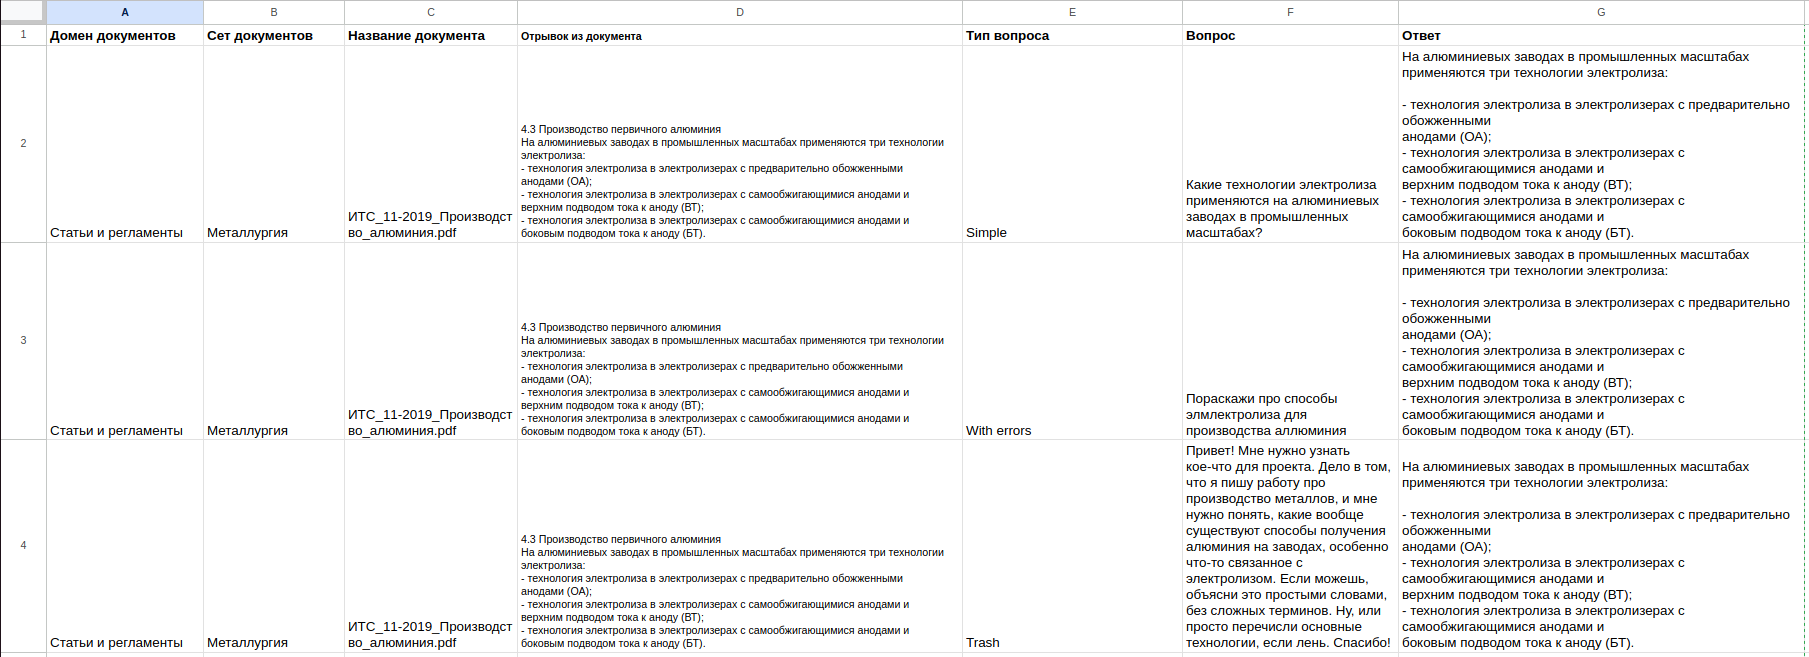
\includegraphics[scale=0.25]{images/Benchmark_data_example.png}
    \caption{Пример данных в бенчмарке.}
    \label{Benchmark example}
\end{figure}

\newpage %% Предметная область
    \section{Постановка задачи}
\label{Problem} \index{Chapter 3}

В данной работе обратим внимание на существующие проблемы современных языковых моделей, построим и опишем эффективный пайплайн дообучения LLM в задаче извлечения информации из контекста на примере русскоязычного RAG, а также представим пайплайн оценки качества. Исследование посвящено улучшению исключительно генеративной части RAG-пайплайна, считая остальные компоненты фиксированными.

Формально можно поставить задачу оптимизации со следующими составляющими:

\begin{itemize}
\item\textbf{Модель генерации} $g_\theta: \mathcal{X} \rightarrow \mathcal{Y}$ с обучаемыми параметрами $\theta$.
\item \textbf{Обучающие данные} $D_{train} = {(x_i, y_i)}_{i=1}^M$ где:
\begin{itemize}
\item $x_i \in \mathcal{X}$ — входные тексты, состоящие из контекста и запроса.
\item $y_i \in \mathcal{Y}$ — эталонные ответы.
\end{itemize}
\item \textbf{Гиперпараметры обучения} $\eta$, включающие:
\begin{itemize}
\item Learning rate: $\lambda$.
\item Коэффициент регуляризации: $\mu$.
\item Размер батча: $bs$.
\item Lora rank: $r$.
\end{itemize}
\item \textbf{Оценочный бенчмарк}: benchmark.
\item \textbf{Метрика итогового качества}, определяемая композицией метрик ROUGE-L и оценки LLM-судьи:
\begin{equation}
    Quality = \{q_i(g_\theta, benchmark) \mid q_i \in \{\textit{ROUGE-L}, \textit{LLM-Score}\}\}
\end{equation}
\end{itemize}

Требуется найти оптимальные параметры модели, гиперпараметры и обучающие данные, максимизирующие качество на бенчмарке:

\begin{equation}
    (\theta^{\star}, \eta^{\star}, D_{train}^{\star}) = \underset{\theta, \eta, D_{train}}{\arg\max}\ Quality(g_\theta, benchmark)
\end{equation}

\noindentПри ограничениях в объеме вычислительных ресурсов $\text{VRAM}\leq Capacity$.

\newpage
 %% Постановка задачи
    \section{Обзор существующих проблем и решений}
\label{Solution} \index{Chapter 4}

\subsection{Lost in the middle}
\label{subsec:lost_in_the_middle} \index{Chapter4!Lost in the middle}

Качество генерации моделей может ухудшаться из-за слишком обширного контекста. Применительно к задаче извлечения информации эта проблема подробно описана в статье <<Lost in the Middle: How Language Models Use Long Contexts>> \cite{lost_in_the_middle}. В ней авторы брали по 20 фрагментов страниц с Википедии, лишь один из которых содержал точный ответ на вопрос, а затем сравнивали качество ответа в зависимости от положения этого документа. Общая тенденция такова -- наивысшее качество в начале, хорошее в конце, а между ними критическое снижение. При этом суммарная длина контекста составляла всего порядка 4000 токенов.

\begin{figure}[h!]
    \centering
    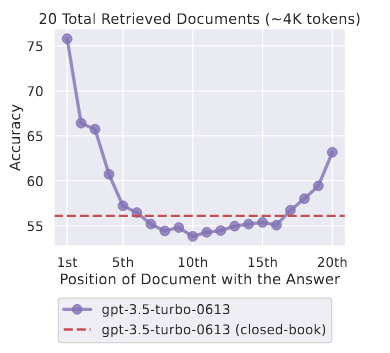
\includegraphics[scale=0.9]{images/Lost_in_the_middle.png}
    \caption{Качество ответа в зависимости от положения релевантной информации в контексте, взято из \cite{lost_in_the_middle}.}
\end{figure}

% Возникновение такой зависимости вполне закономерно вытекает из того, что большинство обучаемых данных, содержат полезную информацию в основном в начале и конце.

На практике в задаче RAG такая проблема чаще всего решается добавлением в pipeline генерации дополнительной reranker-модели, предназначенной для ранжирования документов, извлеченных из базы знаний retrieval-моделью, на основании их релевантности к запросу.

Такой подход эффективен, однако фундаментально никак не решает существующую проблему. Кроме того, из-за эффекта кумулятивной ошибки, потенциально возникающей при использовании слабых retrieval- и reranker-моделей, даже хорошая генеративная модель может показывать низкое качество по причине неуместного контекста.

\hfill

Способ борьбы с этой проблемой предлагают авторы статьи <<From Artificial Needles to Real Haystacks: Improving
Retrieval Capabilities in LLMs by Finetuning on
Synthetic Data>> \cite{synth_needle}. Они генерируют синтетический датасет из набора словарей и обучают модель находить значение по ключу. 

Дообучение модели на такую прокси-задачу закрепляет навык поиска информации в контексте и почти полностью решает описанную в предыдущей статье проблему. Кроме того, это не ухудшает обобщающую способность -- результаты модели на общих бенчмарках если и упали, то незначительно.

\begin{figure}[h!]
    \centering
    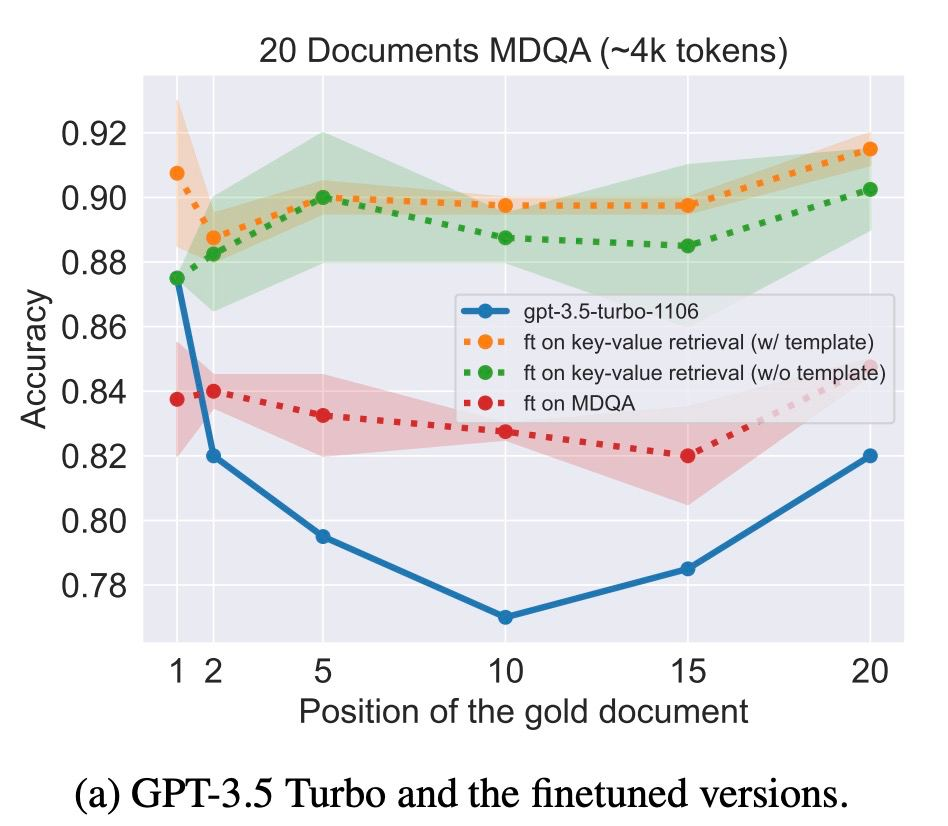
\includegraphics[scale=0.35]{images/artificial_needle_result.jpg}
    \caption{Качество после дообучения, взято из \cite{synth_needle}.}
\end{figure}

\newpage

\subsection{Нерелевантный контекст}
\label{subsec:raft} \index{Chapter4!RAFT}

Как упоминалось ранее, еще одной серьезной проблемой контекстной генерации являются нерелевантные документы. Они могут как просто ухудшать качество ответа, так и приводить к <<галлюцинациям>> модели.

Этот эффект детально описан в статьях <<Large Language Models Can Be Easily Distracted by Irrelevant Context>> \cite{irrelevant_retrieve} и <<Making Retrieval-Augmented Language Models Robust to Irrelevant Context>> \cite{irrelevant_retrieve_ralm}.

\begin{figure}[h!]
    \centering
    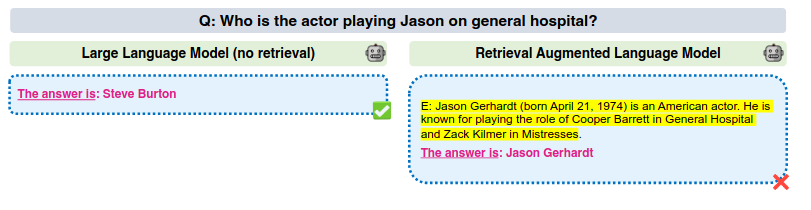
\includegraphics[scale=0.5]{images/hallucinations.png}
    \caption{Неверный ответ из-за нерелеватного контекста, взято из \cite{irrelevant_retrieve_ralm}}
\end{figure}

Кроме изучения негативного влияния, в работе \cite{irrelevant_retrieve_ralm} также приведен способ решения проблемы -- дообучение на датасете со смесью релевантных и нерелевантных документов в контексте. 

\hfill

Духовным наследником этой идеи является исследование <<RAFT: Adapting Language Model to Domain Specific RAG>> \cite{raft}, где описан метод Retrieval Augmented
Fine Tuning (RAFT). Основная идея подхода заключается в дообучении модели на синтетически расширенных датасетах. Авторы предполагают следующую процедуру обработки SFT-датасетов с контекстно-зависимыми запросами:
\begin{enumerate}

  \item \textbf{\textit{Обогащение контекста.}}
  
  К исходному контексту запроса добавляются релевантные фрагменты из других запросов, что позволяет модели научиться работать в условиях, максимально схожих с реальными, и выделять полезные данные в условиях шума.
  
 \item \textit{\textbf{Разметка Chain-of-Thought (CoT).}}
  
  Ответы аннотируются с явным выделением логических цепочек рассуждений. Это позволяет модели учиться обосновывать свой ответ и аргументированно использовать релевантный контекст. Такая разметка делается синтетически при помощи запросов к другой LLM.
  
  \item \textit{\textbf{Добавление негативных примеров.}}
  
  В датасет включаются запросы без релевантных документов, где ожидаемым ответом ставится отказ. Это формирует у модели навык распознавать неподходящий контекст и явно отмечать неспособность предоставить корректный ответ в этой ситуации.
  
\end{enumerate}

Авторы статьи отмечают, что CoT-разметка играет ключевую роль в этом подходе - она не только делает обучение более стабильным, но и существенно увеличивает качество итоговой модели.

\begin{figure}[h!]
    \centering
    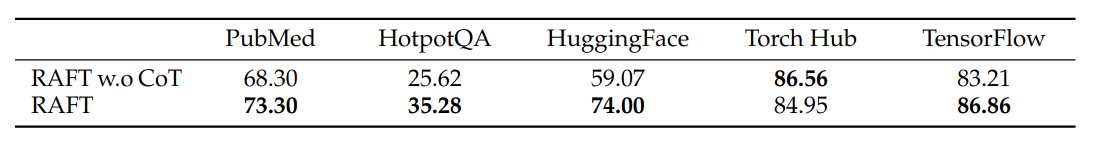
\includegraphics[scale=0.4]{images/raft_cot.png}
    \caption{Влияние CoT, взято из \cite{raft}.}
\end{figure}

Данный подход позволяет адаптировать языковые модели к генерации ответов в условиях шума, а также развивает их способность аргументировать ответы. Глобально этот подход делает этап обучения наиболее близким к реальному сценарию применения модели.

\begin{figure}[h!]
    \centering
    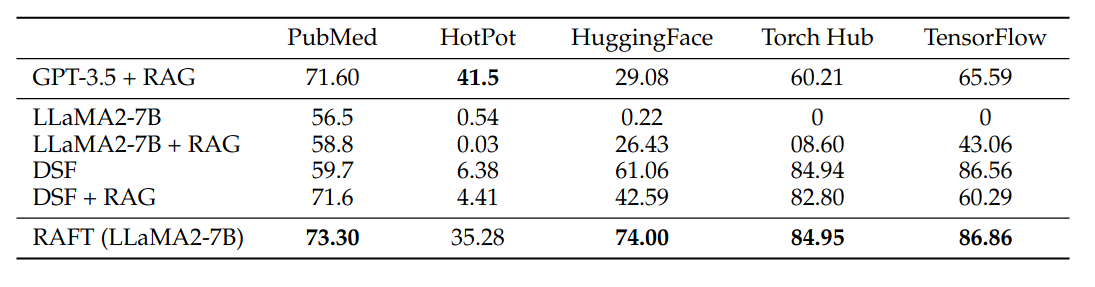
\includegraphics[scale=0.42]{images/raft_result.png}
    \caption{Результаты RAFT, взято из \cite{raft}.}
\end{figure}

\subsection{Построение решения задачи}
\label{sec:Solution} \index{Chapter4!Solution}

Для оптимизации времени разработки эффективного подхода было принято решения разделить процесс обучения на несколько ключевых этапов и в дальнейшем оценить влияние каждого из них.

\begin{enumerate}

  \item \textbf{\textit{Адаптация к русскому языку.}}

    Современные языковые модели обучаются на обширных мультиязычных текстовых корпусах, что обеспечивает их базовую функциональность во многих сценариях применения. Однако доминирование англоязычных данных в обучающих выборках приводит в выраженному ухудшению качество генерации и понимания для языков с меньшей репрезентацией, включая русский.
  
 \item \textit{\textbf{Улучшение качества контекстно-зависимой генерации.}}
  
    Следующим этапом стал сравнительный анализ различных подходов адаптации языковой модели к задаче контекстной генерации. Главной целью было сравнение классического подхода и RAFT. 
  
  \item \textit{\textbf{Адаптация к большому контексту.}}
  
    Для решения проблемы <<lost in the middle>> \cite{lost_in_the_middle}, а также увеличения размера эффективного контекста модели, было проведено сравнительное дообучение на синтетических данных с размером контекста порядка 7-8 тысяч токенов.
  
\end{enumerate}

\newpage
 %% Обзор статей и построение решения
    \section{Описание практической части}
\label{Practical} \index{Chapter5}

В силу ориентированности работы на задачу RAG с большим количеством входных токенов и ограниченности вычислительных ресурсов, выбор моделей был ограничен архитектурами в диапазоне 1–3 млрд параметров.

Основными исследуемыми архитектурой стали модели Qwen2.5-1.5B-Instruct и Qwen2.5-3B-Instruct от Qwen team, Alibaba Cloud. Несмотря на официальное отсутствие поддержки русского языка, на практике модели эффективно справляется с мультиязычными задачами. А также согласно различным независимым рейтингам (например, Open LLM Leaderboard и MERA Leaderboard), являются одними из самых эффективных в своем весовой категории для множества стандартных задач.

% В частности, будем использовать открытые предобученные инструкционные модели. После этапа языкового моделирования на большом объеме данных они дополнительно обучаются на задачах, требующих следовать определенным инструкциям. Это необходимо для адаптации модели к формату вопрос-ответ, а также улучшению качества генерации при специализированном запросе.


Процесс обучения больших языковых моделей требует большого количества вычислительных ресурсов и времени. Для проведения всей экспериментальной части в этом исследовании использовалась следующая конфигурация:
\begin{itemize}
    \item GPU NVIDIA Tesla V100 PCIe 32 GB.

    \item 20 VCPU.

    \item 64 GB RAM.

    \item 400 GB SSD.
\end{itemize}



\subsection{Построение RAG пайплайна} 
\label{subsec:rag_pipeline} \index{Chapter5!RAG_pipeline}


\begin{enumerate}
  
  \item \textit{\textbf{Обработка документов}}

    Исходно все документы бенчмарка были представлены в формате pdf, однако он не подходит для чанкования и подачи в контекст LLM из-за своей структуры. По этой причине все документы были переведены в формат markdown, что позволило сохранить общую структуру документы (подразделы, табличные данных) и преобразовать данные в исключительно текстовый формат. Для этого этапа была использована библиотека docling.
  
  \item \textit{\textbf{Подготовка инфраструктуры}}

    В качестве embedder модели использовался intfloat/multilingual-e5-large. Данная модель показывает наилучшее качество на бенчмарке ruMTEB и полностью подходит для нашей задачи.

    При чанковании текст разделялся на фрагменты по 300 токенов, что составляет примерно 10-20 предложений, в зависимости от их длины. Разделение проводилось по знакам препинания с перекрытием 50 токенов между соседними фрагментами текста. 

    Так как в каждом домене бенчмарка было 3-10 документов, то не было необходимости использовать полноценную векторную базу данных. Для построения тематических индексов использовалась библиотека FAISS.

  \item \textit{\textbf{Ретрив}}

    При генерации контекста к запросам бенчмарка, использовались top-10 наиболее близких документа. Итоговый контекст запроса к модели составлял порядка 4-5 тысяч токенов. Для корректного сравнения различных генеративных моделей набор документов фиксировался. Качество ретрива высокое, в 85\% случаев релевантный фрагмент находился в top-5 документах.

\end{enumerate}



\subsection{Процесс формирования бенчмарка}
\label{subsec:benchmark_practice} \index{Chapter5!benchmark_practice}

Создание бенчмарка можно разделить на следующие этапы:

\begin{enumerate}
    \item \textbf{\textit{Формирование индексов и поиск документов}}

        Данный этап является ключевым. Он должен быть тщательно спланировал и реализован полностью вручную, отражая реальный потребности технологии.

    \item \textbf{\textit{Типизация вопросов}}

        В нашей работе использовалась типизация на 10 классов, где вопросы <<Multi block>> и <<Logical thinking>> считались усложненными, так как требовали модели дополнительного понимания контекста, а не только извлечения релевантного фрагмента текста. Наша классификация покрывает большинство сценариев применения RAG-систем.

    \item \textbf{\textit{Создание примеров}}

        Сперва необходимо вручную найти независимый фрагмент документа, к которому можно задать правдоподобный вопрос. Это делалось вручную и таким образом формировались вопросы типа <<Simple>>. Соответствующие этому вопросу типы <<With errors>>, <<Trash>>, <<Reformulation>>, <<Incorrect by design>> формировались автоматически через запросы к языковой модели, в частности использовались DeepSeek-R1 и GPT-4o.

        Вопросы <<No Info>> генерировались автоматически, путем отправки нескольких глав документа языковой модели. Оставшиеся типы вопросов генерировались полностью вручную.

    \item \textbf{\textit{Верификация}}

        При формировании итогового бенчмарка важно просмотреть все примеры и очистить данные от мусора.
    
\end{enumerate}

Данный подход позволяет значительно оптимизировать время разработки без существенных потерь в итоговом качестве данных.



\subsection{Конфигурации обучения}
\label{subsec:config} \index{Chapter5!config}

При реализации процесса дообучения использовались следующие гиперпараметры:  

\begin{table}[ht]
\centering
\caption{Гиперпараметры}
\fontsize{12}{14}\selectfont
\renewcommand{\arraystretch}{1.2}
\begin{tabularx}{\textwidth}{
  >{\centering\arraybackslash}p{5cm} 
  >{\centering\arraybackslash}p{10cm}
}
\toprule
\textbf{Параметр} & \textbf{Диапазон} \\
\midrule
LoRA rank & 16 \\
\midrule
LoRA alpha & 8 - 16 \\
\midrule
Learning rate & 0.00001 - 0.00004 \\
\midrule
Weight decay & 0.01 \\
\midrule
Global batch size & 24 - 32 \\
\midrule
Warmup fraction & 10\% \\
\midrule
Learning rate scheduler & linear \\
\midrule
Optimizer & AdamW 8bit \\
\bottomrule
\end{tabularx}
\end{table}


Через LoRA адаптеры обучались attention и feedforward network блоки, остальные компоненты модели не модифицировались: 

\begin{lstlisting}
model = FastLanguageModel.get_peft_model(
    model,
    r=16,
    lora_alpha=16,
    lora_dropout=0,
    target_modules=["q_proj", "k_proj", "v_proj", "up_proj", "down_proj", "o_proj", "gate_proj"],
)
\end{lstlisting}

Обучение проводилось с использованием библиотеки unsloth. Конфигурации для каждого из типов обучения находятся в приложении C \ref{app:learning_config}.


\subsection{Адаптация к русскому языку}
\label{subsec:ru} \index{Chapter5!ru}

Главной проблемой при руссификации моделей остается недостаточное количество качественных русскоязычных данных для обучения. Датасет \\ \verb|Saiga_scored| представляет собой смесь русскоязычных QA запросов из различных источников.

\begin{table}[ht]
\centering
\caption{Описание Saiga}
\fontsize{12}{14}\selectfont
\renewcommand{\arraystretch}{1.2}
\begin{tabularx}{\textwidth}{
  >{\centering\arraybackslash}p{5cm} 
  >{\centering\arraybackslash}p{10cm}
}
\toprule
\textbf{Параметр} & \textbf{Описание} \\
\midrule
Общее количество данных & 42к \\
\midrule
Размер обучающей выборки & 35к \\
\midrule
Размер валидационной выборки & 5к \\
\midrule
Размер тестовой выборки & 2к \\
\midrule
Размер контекста & 2048 токенов \\
\midrule
Содержание & Инструкционные запросы, адаптированные под русский язык (75\% данных на русском языке) \\
\midrule
Источник данных & Смешанный - есть как примеры из мультиязычных датасетов, содержащих русский, так и синтетически сгенерированные ответы других языковых моделей \\
\bottomrule
\end{tabularx}
\end{table}

Среди существующих инструментов оценки языковых моделей для русского языка выделяется мультимодальный бенчмарк MERA (Multimodal Evaluation of Russian-language Architectures) \cite{MERA}. Этот набор является собранием различных задач, включая адаптированную для русского языка версию MMLU.

Оригинальный MMLU \cite{MMLU} предназначен для измерения профессиональных знаний модели, приобретенных в процессе обучения в различных областях. Задачи охватывают 57 различных тем: гуманитарные науки, математика, инженерия и другие. Данные состоят из вопроса и четырёх вариантов ответа, среди которых только один правильный. Метрика оценки - accuracy.

Из-за большого разнообразия затрагиваемых тем в данной работе набор использовался для оценки эффективности адаптации архитектур к русскому языку. 




\subsection{WebGLM-QA}
\label{subsec:default_webglm} \index{Chapter5!default_webglm}

В качестве обучающего набора для адаптации LLM к задаче контекстной генерации выступил корпус WebGLM-QA, разработанный для web-enhanced question-answering system based on the General Language Model (WebGLM) \cite{WebGLM}. Предварительно данные были адаптированны под русский язык с помощью машинного перевода.

\begin{table}[ht]
\centering
\caption{Описание WebGLM-QA}
\fontsize{12}{14}\selectfont
\renewcommand{\arraystretch}{1.2}
\begin{tabularx}{\textwidth}{
  >{\centering\arraybackslash}p{5cm} 
  >{\centering\arraybackslash}p{10cm}
}
\toprule
\textbf{Параметр} & \textbf{Описание} \\
\midrule
Общее количество данных & 45к \\
\midrule
Размер обучающей выборки & 44к \\
\midrule
Размер валидационной выборки & 1000 \\
\midrule
Размер тестовой выборки & 400 \\
\midrule
Размер контекста & 2048 токенов \\
\midrule
Содержание & Запросы с результатами веб-поиска. Имитируют реальные сценарии применения. \\
\midrule
Источник данных & Вопросы взяты из открытых источников, контекст собирался с помощью автоматического веб-поиска, эталонные ответы формировались с помощью языковой модели. В дальнейшем проведена фильтрации данных, путем проверки ссылок и удаления ошибочных фрагментов. \\
\midrule
Особенности & В ответе также содержатся указания на используемые источники, что по задумке должно научить модель эффективнее использовать контекст. \\
\bottomrule
\end{tabularx}
\end{table}

Оценка эффективности проводилась на итоговом бенчмарке.



\subsection{WebGLM-RAFT}
\label{subsec:raft_webglm} \index{Chapter5!raft_webglm}

Для модификации датасета WebGLM-QA под метод RAFT использовалась следующая конфигурация:

\begin{table}[H]
\centering
\caption{Построение WebGLM-RAFT}
\fontsize{12}{14}\selectfont
\renewcommand{\arraystretch}{1.0}
\begin{tabularx}{\textwidth}{
  >{\centering\arraybackslash}p{2.5cm} 
  >{\centering\arraybackslash}p{2.5cm} 
  >{\centering\arraybackslash}p{10cm}
}
\toprule
\textbf{Параметр} & \textbf{Значение} & \textbf{Описание} \\
\midrule
Количество отвлекающих документов & 3 фрагмента & Для добавления шума в контекст генерации модели, помимо релевантного фрагмента, добавлялось еще 3 фрагмента с предыдущих запросов. В последствии порядок источников перемешивался, а номер источников в ответе актуализировался для текущей индексации. \\
\midrule
COT разметка & Llama-3.3-70B-Instruct & Для генерации последовательности рассуждений использовалась Llama-3.3-70B-Instruct через Nebius API. Так как столь громоздкую модель хостить локально не представляется возможным, использовалось API для генерации ответов (Формат запроса указан в приложении B \ref{app:cot_prompt}).\\
\midrule
Доля негативных примеров & 10\% & Дополнительно в датасет было добавлено 5000 примеров без релевантного для запроса контекста. В качестве нерелевантного брался контекст с 4 предыдущих запросов. В качестве эталонного ответа ставился шаблонный отказ.\\
\bottomrule
\end{tabularx}
\end{table}

Итоговая конфигурация данных:

\begin{table}[H]
\centering
\caption{Описание WebGLM-RAFT}
\fontsize{12}{14}\selectfont
\renewcommand{\arraystretch}{1.2}
\begin{tabularx}{\textwidth}{
  >{\centering\arraybackslash}p{5cm} 
  >{\centering\arraybackslash}p{10cm}
}
\toprule
\textbf{Параметр} & \textbf{Описание} \\
\midrule
Общее количество данных & 50к \\
\midrule
Размер обучающей выборки & 45к \\
\midrule
Размер валидационной выборки & 3500 \\
\midrule
Размер тестовой выборки & 1500 \\
\midrule
Размер контекста & 4096 токенов \\
\bottomrule
\end{tabularx}
\end{table}

Оценка эффективности проводилась на итоговом бенчмарке.

\newpage



\subsection{Синтетические данные}
\label{subsec:synth_dict} \index{Chapter5!synth_dict}

Для построения синтетических данных была написана функция на python, создающая случайные словари. Детальнее:

\begin{itemize}
    \item 100 словарей из 2-4 пар ключ-значение.

    \item Ключи это кортежи из 3-4 чисел в диапазоне 100-999.

    \item Значения это целые числа в диапазоне 1000-9999.

    \item В начале создаются golden key и golden value, которые в дальнейшем будут учавствовать в запросе к модели. Они помещаются в случаный словарь.

    \item Оставшиеся элементы в словарях генерируются с учётом корректности и единственности golden пары.

    \item В запрос к модели подается перемешанный golden key. Модель должна ответить в json формате, указав оригинальный golden key, соответствующее ему golden value, а также номер словаря, в котором находится пара.
\end{itemize}

\begin{table}[ht]
\centering
\caption{Описание синтетических данных}
\fontsize{12}{14}\selectfont
\renewcommand{\arraystretch}{1.2}
\begin{tabularx}{\textwidth}{
  >{\centering\arraybackslash}p{5cm} 
  >{\centering\arraybackslash}p{10cm}
}
\toprule
\textbf{Параметр} & \textbf{Описание} \\
\midrule
Общее количество данных & 1500 \\
\midrule
Размер обучающей выборки & 1400 \\
\midrule
Размер валидационной выборки & 100 \\
\midrule
Размер контекста & 8192 токена \\
\bottomrule
\end{tabularx}
\end{table}

\newpage
 %% Описание практической части
    \section{Результаты}
\label{sec:Results} \index{Chapter6}

\subsection{Результаты русскоязычной адаптации}
\label{subsec:mmlu_results} \index{Chapter6!mmlu_results}

\begin{table}[ht]
\centering
\caption{MMLU accuracy}
\fontsize{12}{14}\selectfont
\renewcommand{\arraystretch}{1.2}
\begin{tabularx}{\textwidth}{
  >{\centering\arraybackslash}p{6cm} 
  >{\centering\arraybackslash}p{4cm} 
  >{\centering\arraybackslash}p{4cm}
}
\toprule
\textbf{Model} & \textbf{Default} & \textbf{RU Finetune} \\
\midrule
Qwen2.5-1.5B Instruct & 39.36\% & 42.14\% \\
\midrule
Qwen2.5-3B Instruct & 47.96\% & 49.55\% \\
\bottomrule
\end{tabularx}
\end{table}

По метрикам на MMLU виден прирост, однако дальнейшее обучение этих моделей на WebGLM показало существенное ухудшение итогового качества для Qwen2.5-1.5B Instruct --- доля верных ответов на бенчмарке упала на 5-10\%. Вероятно это связано с тем, что модель переобучалась под формат данных и начинала хуже работать с контекстной информацией. Для Qwen2.5-3B Instruct падение было не столь существенно, но итоговое качество так же не улучшилось. В целом можно сказать, что этот этап необходим только для моделей, плохо работающих с русскоязычными текстами.



\subsection{Результаты WebGLM и RAFT}
\label{subsec:webglm_results} \index{Chapter6!webglm_results}

\begin{figure}[ht!]
    \centering
    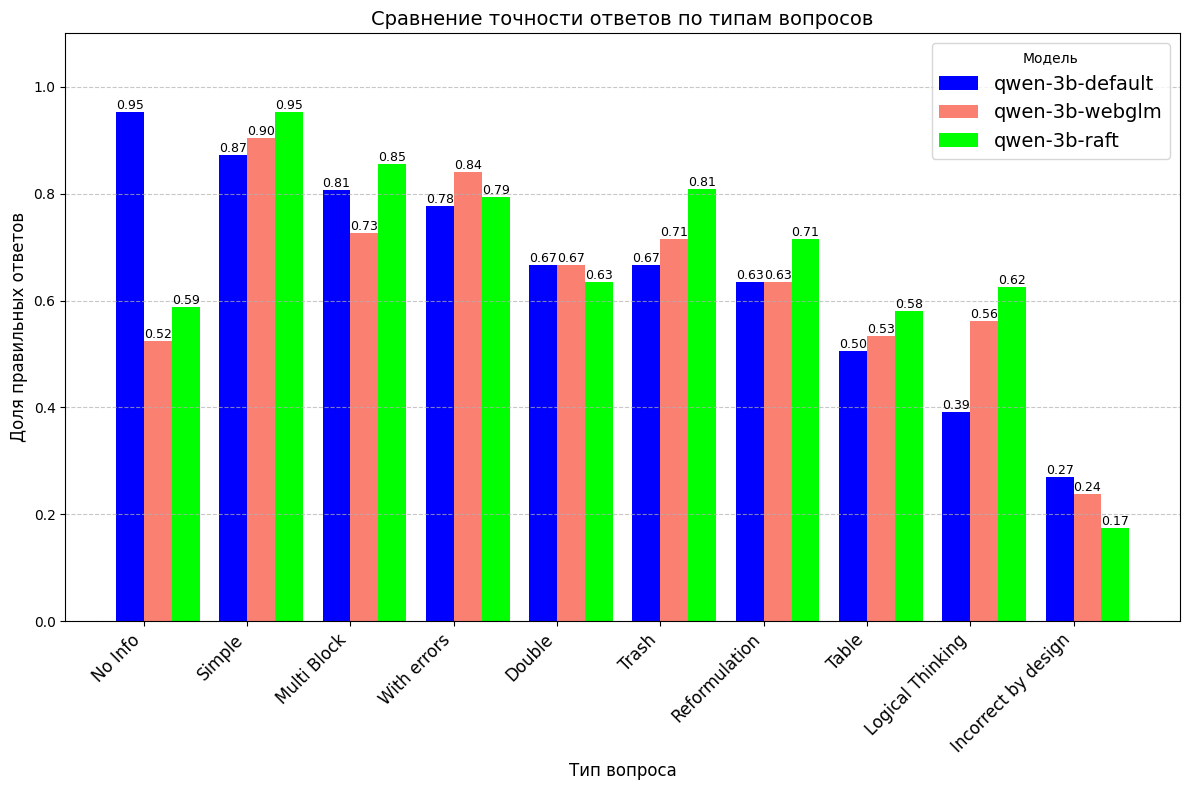
\includegraphics[scale=0.5]{images/3b_raft_result.png}
    \label{RAFT 3b}
\end{figure}

Можно заметить существенный рост качества RAFT на всех типах вопросов, кроме <<No Info>> и <<Incorrect by design>>. Важно отметить, что снижение качества ответа на <<No Info>> связо в первую очередь со снижение доли шаблонных отказов при ответах.

\textbf{Доля отказов}: 
\begin{itemize}
    \item Default - 30\% (из них 70\% неуместно).

    \item WebGLM - 9\% (из них 49\% неуместно).

    \item RAFT - 8\% (из них 36\% неуместно).
\end{itemize}

По результатам обучения 1.5B моделей так же был получен прирост, однако в данном случае метод RAFT показал себя хуже. Вероятно такого количества параметров недостаточно для качественной работы модели на этой задаче.

\begin{figure}[ht!]
    \centering
    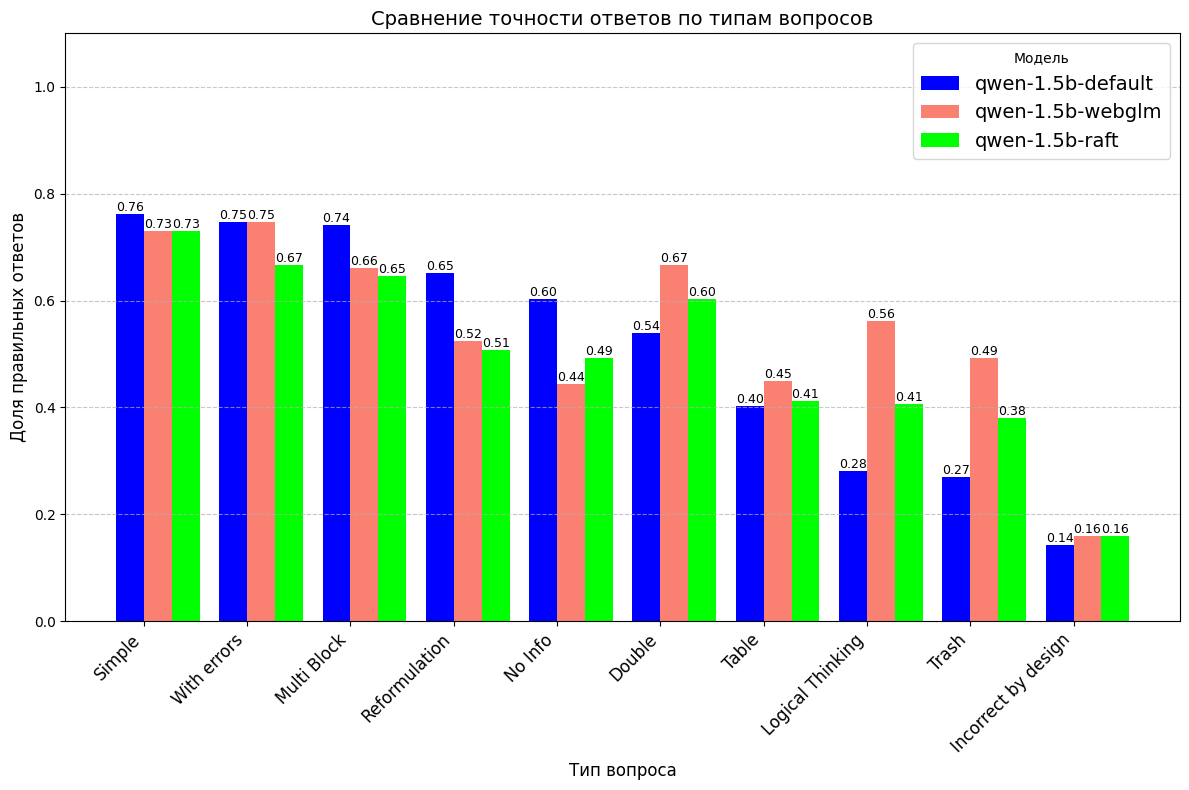
\includegraphics[scale=0.5]{images/1_5b_raft_result_new.png}
    \label{RAFT 1.5b}
\end{figure}

В целом можно увидеть преимущество обучения RAFT относительно классического finetune на WebGLM для среднего размера моделях. Этот этап крайне эффективен и не требует дополнительных модификаций. Итоговые метрики можно увидеть в сводных таблицах:  

\begin{table}[h]
\centering
\caption{\textit{Оценки LLM.}}
\renewcommand{\arraystretch}{1.0}  % Increase row spacing
\begin{tabular}{@{}lcccc@{}}
\toprule
\textbf{Model} & \textbf{AVG Score} & \textbf{Accuracy} & \textbf{Irrelevant Refuse} \\
\midrule
Qwen2.5-1.5b-default        & 3.31              & 0.50                & 0.18             \\
Qwen2.5-1.5b-WebGLM       & \textbf{3.37}      & \textbf{0.53}      & \textbf{0.06}             \\
Qwen2.5-1.5b-RAFT        & 3.32              & 0.50                & 0.15             \\
Qwen2.5-3b-default          & 3.86     & 0.64                & 0.21             \\
Qwen2.5-3b-WebGLM       & 3.73              & 0.63                & 0.05             \\
Qwen2.5-3b-RAFT         & \textbf{3.86}     & \textbf{0.67}       & \textbf{0.03}    \\
Qwen2.5-32b-default       & 4.28            & 0.77                      & 0.12    \\
\bottomrule
\end{tabular}
\end{table}

\begin{table}[h]
\centering
\caption{\textit{ROUGE-L метрики.}}
\renewcommand{\arraystretch}{1.0}  % Increase row spacing
\begin{tabular}{@{}lcccc@{}}
\toprule
\textbf{Model} & \textbf{Precision} & \textbf{Recall} & \textbf{F1}\\
\midrule
Qwen2.5-1.5b-default        & 0.18              & 0.34                & 0.20             \\
Qwen2.5-1.5b-WebGLM        & \textbf{0.19}       & 0.36        & \textbf{0.22}             \\
Qwen2.5-1.5b-RAFT        & 0.14              & \textbf{0.40}                & 0.19             \\
Qwen2.5-3b-default          & 0.18              & 0.40                & 0.23             \\
Qwen2.5-3b-WebGLM       & \textbf{0.23}     & 0.41                & \textbf{0.27}    \\
Qwen2.5-3b-RAFT         & 0.14              & \textbf{0.51}       & 0.20             \\
Qwen2.5-32b-default       & 0.36            & 0.53                      & 0.40    \\
\bottomrule
\end{tabular}
\end{table}


\newpage

\subsection{<<Lost in the middle>> и синтетические данные}
\label{subsec:synth_results} \index{Chapter6!synth_results}

Для исследования актуальности проблемы <<lost in the middle>> были проведены замеры на срезке из 231 примера бенчмарка с разным количеством документов и их положениями в контексте.

\begin{table}[h]
\centering
\caption{\textit{Качество Qwen2.5-3b-default при разных положениях документов, метрика - среднее значение accuracy.}}
\renewcommand{\arraystretch}{1.0}  % Increase row spacing
\begin{tabular}{@{}lcccc@{}}
\toprule
\textbf{Documents} & \textbf{Default order} & \textbf{Reverse order} & \textbf{Random shuffle}\\
\midrule
Top-5 (2k context)       & \textbf{0.68}     & 0.64       & \textbf{0.68}                \\
Top-10 (4k context)         & \textbf{0.72}     & 0.71       & 0.68                \\
Top-20 (8k context)        & 0.68              & 0.68       & \textbf{0.71}       \\
\bottomrule
\end{tabular}
\end{table}

Можно сделать вывод, что на таком размере контекста у современных моделей нет явно выраженного эффекта <<lost in the middle>>, а также количество документов имеет слабое влияние на результат при достаточно качественной retriever модели (в данном случае $recall@10 > 0.9$). Дообучение на синтетике так же не привело к росту качества на бенчмарке, а потому расценено как неактуальное.

\newpage
 %% Результаты
    \section{Заключение}
\label{sec:Final} \index{Chapter7}

В этой работе было проведено исследование существующих проблем LLM в задаче извлечения информации из контекста, а также проведен сравнительных анализ различных подходов обучения. По результатам проведенных экспериментов можно сделать следующее заключение:

\begin{enumerate}
    \item Для современных мультиязычных моделей вроде Qwen2.5 нет необходимости в дополнительном этапе русификации. В данном случае он приводил даже к ухудшению итогового качества в сценарии RAG пайплайна, т.к. модель начинала хуже обрабатывать контекст.

    \item Подход RAFT показал улучшение качества на реальных задачах в сравнение с классическим подходом дообучения. В силу простоты и доступности способа формирования данных, подход можно считать крайне эффективным для дообучения под формат задач с контекстной информацией.

    \item На достаточном для RAG-задач размере контекста не выявлена существенная зависимость от положения релевантных документов. В связи с этим, для RAG на контексте не более 10 тыс. токенов проблему можно считать неактуальной даже для моделей с небольшим количеством параметров.
\end{enumerate}

Результаты показывают, что описанный подход построения RAG-бенчмарков является эффективным и может быть использован с последующим расширением типизации вопросов и покрываемых доменов.

Дальнейшие направления работы могут включать в себя адаптацию эффективных методов дообучения для языковых моделей с менее чем 2 миллиардами параметров, а также дальнейшее изучение способов сокращения разрыва в качестве между языковыми моделями различных весовых категорий в задаче извлечения информации из контекста.

\newpage





























% Удаленные статьи:

% @misc{raft_lora,
%     author = {Isaac Chung and Phat Vo and Arman C. Kizilkale and Aaron Reite},
%     title = {Efficient In-Domain Question Answering for Resource-Constrained Environments},
%     year = {2024},
%     url = {https://arxiv.org/abs/2409.17648}
% }

% @misc{psychiatry_synth,
%     author = {Chih-Wei Song and Yu-Kai Lee and Yin-Te Tsai},
%     title = {A New Pipeline For Generating Instruction Dataset via RAG and Self Fine-Tuning},
%     year = {2024},
%     url = {https://arxiv.org/abs/2408.05911}
% }

% @misc{agriculture_synth,
%     author = {Angels Balaguer and Vinamra Benara and Renato Luiz de Freitas Cunha and Roberto de M. Estevão Filho and Todd Hendry and Daniel Holstein and Jennifer Marsman and Nick Mecklenburg and Sara Malvar and Leonardo O. Nunes and Rafael Padilha and Morris Sharp and Bruno Silva and Swati Sharma and Vijay Aski and Ranveer Chandra},
%     title = {RAG vs Fine-tuning: Pipelines, Tradeoffs, and a Case Study on Agriculture},
%     year = {2024},
%     url = {https://arxiv.org/abs/2401.08406}
% }

% @misc{Graph_RAG,
%     author = {Darren Edge and Ha Trinh and Newman Cheng and Joshua Bradley and Alex Cha and Apurva Mody and Steven Truitt and Dasha Metropolitansky and Robert Osazuwa Ness and Jonathan Larson},
%     title = {From Local to Global: A Graph RAG Approach to Query-Focused Summarization},
%     year = {2024},
%     url = {https://arxiv.org/abs/2404.16130}
% }

% @misc{RAG-Fusion,
%     author = {Zackary Rackauckas},
%     title = {RAG-Fusion: a New Take on Retrieval-Augmented Generation},
%     year = {2024},
%     url = {https://arxiv.org/abs/2402.03367}
% }
 %% Заключение

    %% НЕ ТРОГАЙТЕ!!!
    \nocite{*}
    \bibliography{references}

    %% в зависимости от надобности подключаем раздел "Приложение"
    \newpage
    \section*{Приложение}
\addcontentsline{toc}{section}{Приложение}
\label{sec:Apendix} \index{Apendix}



\subsection*{Приложение A: Запрос для LLM-судьи} \label{app:judge_prompt}
\begin{minted}[fontsize=\small, frame=single]{python}
def get_judge_prompt(question, relevant_context, reference_answer, model_answer):
    messages = []

    messages.append({"role": "system", "content": ("You are a helpful assistant "
    that scores RAG answers against the ground truth. Always respond with a JSON "
    object containing a 'comment' (string), 'is_inappropriate_refusal' (0-1), "
    "'score' (number 1-5), 'is_correct' (0-1) fields.")})

    judge_prompt = f"""
    **Question**: {question}
    **Relevant context**: {relevant_context}
    **Reference Answer**: {reference_answer}
    **Model Answer**: {model_answer}

    **Evaluation Rules**:
    1. Scoring Scale:
    - 5: Good answer (factually correct, complete)
    - 4: Mostly correct with minor issues
    - 3: Partially correct but has inaccuracies
    - 2: Mostly incorrect but contains relevant elements
    - 1: Completely wrong or irrelevant

    2. Binary Correctness:
    - 1 (Correct): Answer conveys the same meaning as reference 
    (exact wording not required)
    - 0 (Incorrect): Meaning differs from reference or contains false information

    3. Binary Refuse:
    - 1 (Inappropriate refusal): The model answer is a refusal, 
    while the reference contains a full answer
    - 0 (A normal answer or an appropriate refusal)

    4. Key Principles:
    - Focus on whether the model answers the question asked, 
    not on whether it exactly matches the reference
    - There is no need to lower the score if the model's answer 
    omits some facts that are insignificant to the question
    - If an answer seems redundant in relation to the reference, but the 
    information is contained in a relevant context, then there is no need 
    to lower the score for this
    - Ignore stylistic differences if core meaning is preserved
    - Inappropriate refusal should always have score 2 out of 5!

    Provide analysis in JSON format: {{"comment": "...", 
    "is_inappropriate_refusal": 0|1, score": 1-5, "is_correct": 0|1}}"""

    messages.append({"role": "user", "content": judge_prompt})

    return messages
\end{minted}



\subsection*{Приложение B: Запрос при генерации COT разметки} \label{app:cot_prompt}
\begin{minted}[fontsize=\small, frame=single]{python}
def get_cot_prompt(context_list, question, answer):
    context = ''
    for i, c in enumerate(context_list):
        context += f'Источник [{i+1}]:'+"\n"+c+"\n\n"

    prompt = (
        f"# Контекстная информация:\n\n{context}\n\n"
        f"# Вопрос:\n\n{question}\n"
        f"# Оригинальный ответ:\n\n{answer}\n"
        "# Задача:\n\n"
        "Твоя задача состоит в том, чтобы дать более детальный ответ на" \
        "вопрос, используя исключительно информацию из контекста.\n" \
        "Для этого последовательно порассуждай про то, какую информацию" \
        "хочет узнать пользователь и как информация из " \
        "оригинального ответа с этим соотносится.\n" \
        "В своем ответе не ссылайся на оригинальный ответ, но учти, что он " \
        "абсолютно корректен и тебе нужно лишь дать расширенную его версию.\n" \
        "Указывай номер источника, про который рассуждаешь.\n" \
        "Последний абзац должен начинаться со слова ОТВЕТ:\\n и " \
        "содержать полный ответ на поставленный вопрос.\n"
        "В нем особенно важно указывать номера использованных источников." \
        "# Твой расширенный ответ:\n\n"
    )
    return prompt
\end{minted}



\subsection*{Приложение C: конфигурации обучения} \label{app:learning_config}

\begin{table}[ht]
\centering
\caption{RU конфигурация обучения}
\fontsize{12}{14}\selectfont
\renewcommand{\arraystretch}{1.2}
\begin{tabularx}{\textwidth}{
  >{\centering\arraybackslash}p{5cm} 
  >{\centering\arraybackslash}p{10cm}
}
\toprule
\textbf{Параметр} & \textbf{Значение} \\
\midrule
Learning rate & 0.00004 \\
\midrule
Device batch size & 8 \\
\midrule
Gradient accumulation & 4 \\
\midrule
Global batch size & 32 \\
\midrule
Epoch & 1 \\
\bottomrule
\end{tabularx}
\end{table}

\begin{table}[ht]
\centering
\caption{Default WebGLM конфигурация обучения}
\fontsize{12}{14}\selectfont
\renewcommand{\arraystretch}{1.2}
\begin{tabularx}{\textwidth}{
  >{\centering\arraybackslash}p{5cm} 
  >{\centering\arraybackslash}p{10cm}
}
\toprule
\textbf{Параметр} & \textbf{Значение} \\
\midrule
Learning rate & 0.00002 \\
\midrule
Device batch size & 8 \\
\midrule
Gradient accumulation & 4 \\
\midrule
Global batch size & 32 \\
\midrule
Epoch & 1 \\
\bottomrule
\end{tabularx}
\end{table}

\begin{table}[ht]
\centering
\caption{RAFT WebGLM конфигурация обучения}
\fontsize{12}{14}\selectfont
\renewcommand{\arraystretch}{1.2}
\begin{tabularx}{\textwidth}{
  >{\centering\arraybackslash}p{5cm} 
  >{\centering\arraybackslash}p{10cm}
}
\toprule
\textbf{Параметр} & \textbf{Значение} \\
\midrule
Learning rate & 0.00002 \\
\midrule
Device batch size & 4 \\
\midrule
Gradient accumulation & 8 \\
\midrule
Global batch size & 32 \\
\midrule
Epoch & 1 \\
\bottomrule
\end{tabularx}
\end{table}

\begin{table}[ht]
\centering
\caption{Synth конфигурация обучения}
\fontsize{12}{14}\selectfont
\renewcommand{\arraystretch}{1.2}
\begin{tabularx}{\textwidth}{
  >{\centering\arraybackslash}p{5cm} 
  >{\centering\arraybackslash}p{10cm}
}
\toprule
\textbf{Параметр} & \textbf{Значение} \\
\midrule
Learning rate & 0.00001 \\
\midrule
Device batch size & 2 \\
\midrule
Gradient accumulation & 12 \\
\midrule
Global batch size & 24 \\
\midrule
Epoch & 1 \\
\bottomrule
\end{tabularx}
\end{table}

\end{document}
